\clearpage
\subsubsection{\olly + \RU{упаковка полей по умолчанию}\EN{fields are packed by default}}
\index{\olly}

\RU{Попробуем в \olly наш пример, где поля выровнены по умолчанию (4 байта)}
\EN{Let's try our example (where the fields are aligned by default (4 bytes)) in \olly}:

\begin{figure}[H]
\centering
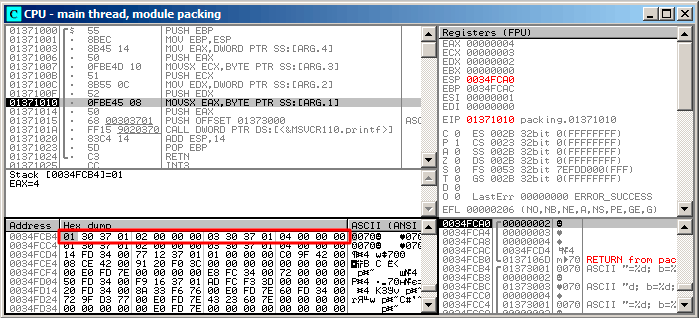
\includegraphics[scale=\FigScale]{patterns/15_structs/4_packing/olly_packing_4.png}
\caption{\olly: \RU{Перед исполнением \printf}\EN{Before \printf execution}}
\label{fig:packing_olly_4}
\end{figure}

\RU{В окне данных видим наши четыре поля}\EN{We see our 4 fields in the data window}.
\RU{Вот только, откуда взялись случайные байты (0x30, 0x37, 0x01) рядом с первым (a) и третьим (c) полем?}
\EN{But where do the random bytes (0x30, 0x37, 0x01) come from, that are next to the first (a) and third (c) fields?}
\RU{Если вернетесь к листингу \myref{src:struct_packing_4}, то увидите, что первое и третье поле имеет
тип \Tchar, а следовательно, туда записывается только один байт, 1 и 3 соответственно (строки 6 и 8).}
\EN{By looking at our listing \myref{src:struct_packing_4}, we can see that the first and third fields
are \Tchar, therefore only one byte is written, 1 and 3 respectively (lines 6 and 8).}
\RU{Остальные три байта 32-битного слова не будут модифицироваться в памяти!}
\EN{The remaining 3 bytes of the 32-bit words are not being modified in memory!}
\RU{А, следовательно, там остается случайный мусор.}\EN{Hence, random garbage is left there.}
\index{x86!\Instructions!MOVSX}
\RU{Этот мусор никак не будет влиять на работу \printf,
потому что значения для нее готовятся при помощи инструкции \MOVSX, которая загружает
из памяти байты а не слова}
\EN{This garbage doesn't influence the \printf output in any way, because the values for it are prepared
using the \MOVSX instruction, which takes bytes, not words}: 
\lstref{src:struct_packing_4} (\RU{строки}\EN{lines} 34 \AndENRU 38).

\RU{Кстати, здесь используется именно \MOVSX (расширяющая знак), потому что тип 
\Tchar\EMDASH{}знаковый по умолчанию в MSVC и GCC.}
\EN{By the way, the \MOVSX (sign-extending) instruction is used here, because 
\Tchar is signed by default in MSVC and GCC.}
\RU{Если бы здесь был тип}\EN{If the type} \TT{unsigned char} \OrENRU \TT{uint8\_t}\EN{ was used here}, 
\RU{то здесь была бы инструкция \MOVZX}\EN{\MOVZX instruction would have been used instead}.

\clearpage
\subsubsection{\olly + \RU{упаковка полей по границе в 1 байт}\EN{fields aligning on 1 byte boundary}}
\index{\olly}

\RU{Здесь всё куда понятнее: 4 поля занимают 10 байт и значения сложены в памяти друг к другу}
\EN{Things are much clearer here: 4 fields occupy 10 bytes and the values are stored side-by-side}

\begin{figure}[H]
\centering
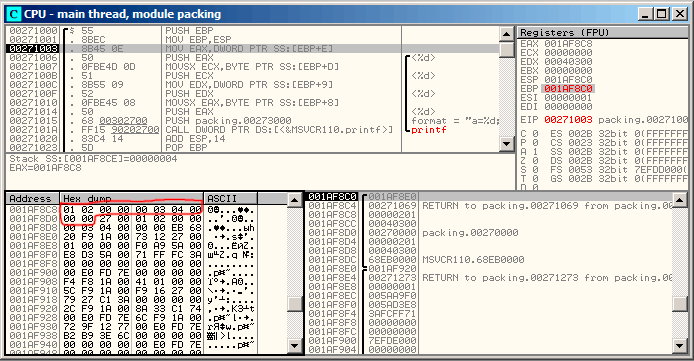
\includegraphics[scale=\FigScale]{patterns/15_structs/4_packing/olly_packing_1.png}
\caption{\olly: \RU{Перед исполнением \printf}\EN{Before \printf execution}}
\label{fig:packing_olly_1}
\end{figure}
